% A template for an Honours Thesis in English Language, NUS: adapted from one by Derek Lim (2016), itself adapted from a template for Carleton College comps papers by Andrew Gainer-Dewar (2013). 
% This work is licensed under the Creative Commons Attribution 4.0 International License.
% To view a copy of this licence, visit http://creativecommons.org/licenses/by/4.0/ or send a letter to Creative Commons, 444 Castro Street, Suite 900, Mountain View, California, 94041, USA.
\documentclass[twoside]{memoir}
\usepackage{nus-el-ht}

% The Latin Modern font is a modernised replacement for the classic Computer Modern. Feel free to replace this with a different font package.
\usepackage{lmodern}
% Hyperref enables click-through hyperlinks in your PDF. The hyphens option indicates where to break long URLs. 
\PassOptionsToPackage{hyphens}{url}\usepackage{hyperref}
% We use setspace to implement double-spacing, but with a specific command to leave quotes single-spaced. 
\DisemulatePackage{setspace}\usepackage{setspace}
\expandafter\def\expandafter\quote\expandafter{\quote\singlespacing}
	\doublespacing

% tikz stuff
\usepackage[usenames,dvipsnames]{color}    
\usepackage[table]{xcolor}
\usepackage{themecolors}
\usepackage{tikz} 
\usetikzlibrary{positioning, shapes.multipart, arrows, arrows.meta, shadows, backgrounds, fit}

% code blocks
\usepackage{listings}
\lstdefinelanguage{isabelle}{%
    keywords=[1]{type_synonym,datatype,fun,abbreviation,definition,proof,lemma,theorem,session,sessions,theories,text,section},
    keywordstyle=[1]\bfseries\color{isabelleouterblue},
    keywords=[2]{where,assumes,shows,and},
    keywordstyle=[2]\bfseries\color{isabelleoutergreen},
    keywords=[3]{if,then,else,case,of,SOME,let,in,O},
    keywordstyle=[3]\color{isabelleinnerblue},
    keywords=[4]{apply, by, done},
    keywordstyle=[4]\color{isabelleoutersalmon},
    morestring=[b]",
    morecomment=[n]{(*}{*)},
    % morecomment=[n]{\guilsingleft}{\guilsingright},
    stringstyle=\color{isabellequote},
    showstringspaces=false,
}
\lstdefinelanguage{file}{
}
\lstset{%
  language=isabelle,
  escapeinside={&}{&},
  columns=fixed,
  extendedchars,
  basewidth={0.5em,0.45em},
  basicstyle=\ttfamily,
  mathescape,
}


% For typesetting and labelling examples, incl. glossed examples. 
% \usepackage{expex} 
% 	\lingset{Everyex=\singlespace}

% Titling commands. 
\title{Stacking Correspondence: Towards Formal Verification of a Network Stack}
\author{Daniel Neshyba-Rowe}
\supervisor {Alain K{\"a}gi}
\degree{Bachelor of Arts with Honors}
\faculty{Mathematical Sciences faculty} % TODO: figure out if this is right
\dept{Computer Science} % TODO: should this be CS and Math?
% \date % TODO: set date?

\begin{document}
% First, we go into "front matter" mode.
% Among other things, this gives us Roman page numbers.
\frontmatter

% We tell LaTeX to make a title page, sections for acknowledgements, the abstract, and the table of contents (important!). 

\maketitle

\chapter{Acknowledgement}
`This page is for making acknowledgements that have a direct bearing on the HT and is not for indulging in routine gestures of politeness or sentimental attitudinising. In all things, the candidate should be guided by good taste and good sense' \pgcitep{data-refinement}{2}. % Note also the command for citing a source and a page number. 

\begin{abstract}
  % citations look like \citep{ell-ht-format}.
      %   Prior work led to the first proven-reliable and viable microkernel, seL4.
      % We hypothesize that similar reliability is possible for a performant IoT device.
      % As a proof of concept, we are creating a networked fish tank thermometer
      % with a complete IPv6 network stack and formally verifying all components.
      %
      % \begin{itemize}
      %     \item should be written for a more general audience
      %     \item alternatively: provide an additional plain-language summary
      % \end{itemize}
      % The job of a microkernel (or operating system) is to share resources
      % between different processes, including CPU time.
      % For a long time, it was thought that the operation of a microkernel was too complex for
      % any kind of formal verification in practice (concurrency makes this particularly tricky).
      % However, the seL4 foundation proved this wrong by creating and verifying the seL4 microkernel, and in doing so opened the gate for future research.
      % In our ongoing project, we hypothesize that the work of seL4 can be extended
      % to a fully-functional, verified embedded system, and attempt to build and
      % verify such a system.
      % For this thesis, we narrow the scope to just consider a piece of the networking stack (the UDP layer), and working on the verification for that piece.
      % In order to do this, we must formally define how we expect the UDP layer to work,
      % defining which behaviors are acceptable and which are not.
      % Subsequently, we must show that our implementation in fact conforms to these expectations.

      In 2009, the seL4 microkernel was released as the first
      industry-grade microkernel which was formally verified to be correct.
      In our work, we hypothesize that it is possible
      to leverage seL4 to create a fully-functional embedded system application running IPv6
      that is verified at all software levels---something thought to be
      practically impossible prior to the release of seL4.
      In our previous work, we designed and built the C code for a networked
      fish tank thermometer as a proof-of-concept of nontrivial complexity.
      Much of the complexity lies in the network stack, which consists of a number of components.
      Here, we focus on the components of the network stack that constitute the UDP layer, continuing the verification process
      by formally defining specifications and refinement steps,
      and applying them to the UDP layer.
      More specifically, we define how we expect the UDP layer to
      work in an abstract specification, describing
      what behaviors are acceptable and which are not.
      Subsequently, we show that the design specification
      of our implementation conforms to these expectations.
      % TODO: note that in fact we do NOT show NADA


\end{abstract}

\tableofcontents

% Include the list of figures and list of tables only if you actually have figures and tables! (The * after each indicates that it should not be included in the table of contents.)
%\listoffigures*
%\listoftables*

% Next, we go into "main matter" mode.
% This resets the page numbers and uses Arabic numerals.
\mainmatter

\chapter{Introduction}

TODO: do I need a motivation?

\section{Background}

This project sits within a larger body of work by seL4 (TODO: citation needed) and K{\"a}gi (TODO: citation needed).
Specifically, some exposition is needed to clarify the process of
formal verification, as well as describe the network stack.
The end goal of this project is to produce a fully functional
networked temperature sensor which records data from a fish tank,
and sends that data over the network where it will be recorded externally.
Furthermore, the goal is to formally show that all software in the
thermometer works correctly, without any bugs or flaws that could cause
it to break or report incorrect data (barring physical malfunctions of the hardware).

\section{Network stack}
Key to a networked temperature sensor is the code responsible for networking---communicating over the internet to other devices.
The standard protocol for network communication is defined in
a variety of RFC and IEEE specifications.
While most of the details are beyond the scope of this paper
(though not the project as a whole), the basic architecture merits some
discussion.

The Open Systems Interconnection (OSI) model describes the standard
implementation of the network stack, for use in communication between
devices.
The network stack is divided into logical layers.
Each layer has a plain-language specification
consisting of either a Request For Comment (RFC) or an IEEE document
that describes the standard interface for interacting with that layer.
At a minimum, each layer contains a \textit{wrap} and an \textit{unwrap}
endpoint, though IP and UDP in particular require more functionality.
As such, we can think of the network stack as a series of composable
encoders and decoders,
where the call to decode a packet might look like
\lstinline{udp_unwrap(ip_unwrap(eth_unwrap(hardware_packet)))}.

If everything works perfectly, then after a packet is encoded
and sent over the physical transmission medium, decoding it should
result in the same packet, unaltered.
One of the principal design features of the OSI model is that since
it is layered, this statement need only apply within a particular layer.
That is, we expect that if we call
\lstinline{y := udp_wrap(x)}, then \lstinline{z := udp_wrap(y)} should
result in the unwrapped packet \lstinline{z} being exactly equal to
the initial packet \lstinline{x}.
If we treat them as functions, we can say that \lstinline{udp_wrap} is 
the inverse function of \lstinline{udp_wrap}.
% TODO: is this notation understandable? Feels somewhat clunky.

\begin{figure}[htpb]
    \centering
    \begin{tikzpicture}[node distance=4cm]
        % styles
        \tikzstyle{cell} = [rectangle, minimum width=4.6cm, minimum height=1cm, text centered, draw=black]
        \tikzstyle{arrow} = [line width=2pt,->,>=latex,draw=gray]
        \tikzstyle{box} = [draw, rectangle, align=center, minimum width=11cm, inner sep=3ex]

        % wrap
        \node (app_wrap) [cell, fill=application!80] {Application on Computer A};
        \node (udp_wrap) [cell, fill=udp!80, below=30pt of app_wrap] {UDP wrap};
        \node (ip_wrap) [cell, fill=ip!80, below=30pt of udp_wrap] {IP wrap};
        \node (ethernet_wrap) [cell, fill=ethernet!80, below=30pt of ip_wrap] {Ethernet wrap};
        \node (hardware_wrap) [cell, fill=hardware!80, below=30pt of ethernet_wrap] {Hardware};

        % unwrap
        \node (app_unwrap) [cell, fill=application!80, right=14pt of app_wrap] {Application on Computer B};
        \node (udp_unwrap) [cell, fill=udp!80, below=30pt of app_unwrap] {UDP unwrap};
        \node (ip_unwrap) [cell, fill=ip!80, below=30pt of udp_unwrap] {IP unwrap};
        \node (ethernet_unwrap) [cell, fill=ethernet!80, below=30pt of ip_unwrap] {Ethernet unwrap};
        \node (hardware_unwrap) [cell, fill=hardware!80, below=30pt of ethernet_unwrap] {Hardware};

        % layers
        \node[box, label={left:\rotatebox{90}{Higher-level}}, fit = (app_wrap) (app_unwrap)] (1) {};
        \node[box, label={left:\rotatebox{90}{Transport}}, fit = (udp_wrap) (udp_unwrap)] (1) {};
        \node[box, label={left:\rotatebox{90}{Network}}, fit = (ip_wrap) (ip_unwrap)] (1) {};
        \node[box, label={left:\rotatebox{90}{Data Link}}, fit = (ethernet_wrap) (ethernet_unwrap)] (1) {};
        \node[box, label={left:\rotatebox{90}{Physical}}, fit = (hardware_wrap) (hardware_unwrap)] (1) {};

        % flow of information
        \draw [arrow] (app_wrap) -- (udp_wrap);
        \draw [arrow] (udp_wrap) -- (ip_wrap);
        \draw [arrow] (ip_wrap) -- (ethernet_wrap);
        \draw [arrow] (ethernet_wrap) -- (hardware_wrap);
        \draw [arrow] (hardware_wrap) -- (hardware_unwrap);
        \draw [arrow] (hardware_unwrap) -- (ethernet_unwrap);
        \draw [arrow] (ethernet_unwrap) -- (ip_unwrap);
        \draw [arrow] (ip_unwrap) -- (udp_unwrap);
        \draw [arrow] (udp_unwrap) -- (app_unwrap);
    \end{tikzpicture}

    
    \caption{A simplified OSI model, showing the wrap and unwrap components of each layer. Arrows show flow of data. Session, presentation, and application layers are combined into a single ``higher-level'' layer---these layers are unnecessary for our use case of a simple thermometer.}
    \label{fig:network-stack}
\end{figure}

\section{seL4}

TODO: look over seL4 paper and make this paragraph more correct:

The seL4 microkernel (TODO: citation needed) is a verified microkernel
that is performant and secure.
The seL4 microkernel provides two important isolation abstractions:
protection domains (PDs),
which can be loosely described as address spaces that provide isolation from
other processes,
and memory regions, which are blocks of physical memory.
Any number of PDs can be associated with a given memory region,
allowing for transfer of data between two PDs 
(see blue box at top of figure~\ref{fig:sel4-mem-pd}),
or storage of data within
a single PD
(see cyan and green boxes at bottom of figure~\ref{fig:sel4-mem-pd}).
Additionally, seL4 provides a notification API,
% TODO: check if this is base seL4 or microkit
whereby a PD can notify a second PD, and the second can,
on receipt of that notification, execute some command.

\begin{figure}[htpb]
    \centering
    \begin{tikzpicture}[node distance=4cm]
        % styles
        \tikzstyle{cell} = [rectangle, minimum width=4.6cm, minimum height=3cm, text centered, draw=black]
        \tikzstyle{arrow} = [line width=2pt,->,>=latex,draw=gray]
        \tikzstyle{box} = [draw, rectangle, align=center, minimum width=11cm, inner sep=3ex]

        % wrap
        \node (mem0) [cell, fill=blue!80] {\LARGE shared memory region};
        \node (PD1) [cell, fill=cyan!80, below left=20pt of mem0] {\LARGE Protection Domain};
        \node (PD2) [cell, fill=green!80, below right=20pt of mem0] {\LARGE Protection Domain};
        \node (mem1) [cell, fill=cyan!80, below=60pt of PD1] {\LARGE memory region}; 
        \node (mem2) [cell, fill=green!80, below=60pt of PD2] {\LARGE memory region}; 
        \node [color=red] at (0, -150pt) {blocked access};
        \node [color=green!200] at (-115pt, -180pt) {good access};

        % flow of information
        \draw [arrow, <->] (PD1) -- (PD2) node[midway, above] {notification};
        \draw [arrow, draw=green] (PD1) -- (mem1);
        \draw [arrow, draw=green] (PD2) -- (mem2);
        \draw [arrow, draw=green] (PD1) -- (mem0);
        \draw [arrow, draw=green] (PD2) -- (mem0);
        \draw [arrow, draw=red!40, -{> Square[black]}] (PD1) -- (mem2);
        \draw [arrow, draw=red!40, -{> Square[black]}] (PD2) -- (mem1);
    \end{tikzpicture}
    \caption{A depiction of some core components of the seL4 microkernel.
    Protection Domains (PDs) can be associated with memory regions,
    and are only able to read or modify those memory regions.
    Additionally, PDs can communicate with each other through notifications.}
    \label{fig:sel4-mem-pd}
\end{figure}
% TODO: make sure this all sounds good

% TODO: split up into assumption and discussion sections?
For the purposes of this paper, we will operate under the assumption that
the UDP layer exists in a completely isolated PD, meaning
we disallow arbitrary (TODO: random?) changes to state by other processes;
the only state changes that occur should be ones initiated by the UDP
layer itself.
In the broader picture of things, we plan to experiment with putting
each layer in a separate PD,
with shared memory regions between adjacent layers to facilitate transfer of data.
In this case, the assumption that state will not be changed by outside processes
need only be relaxed within those shared memory regions, where
data can be written or read from either of the adjacent layers at any time.
This case will necessitate some proof that the behaviors of the two layers
do not interfere within this shared region.
Standardizing information flow using a system of queues along with 
communicating sequential processes (TODO: citation needed)
will likely be useful in this case.

TODO: could mention that putting them all into the same PD could make performance
better, but proofs harder
%
% \subsection{Notation} % maybe combine with the tools section?
% TODO: remove this section, I think
% \begin{itemize}
%     \item refinement
%     \item Hoare triples (TODO: figure out right notation)
%         \[
%         \{|
%             \lambda s. 
%         |\}
%         .\] 
%
%     \item big semantics:
%         \[
%             (c,s) \Rightarrow t
%         \] 
%         means ``command $c$ starting from state $s$ results in state $t$.''
%     \item small step semantics
%     \item $\Gamma$? Not sure yet
%     \item $\top \equiv \lambda s. true$ and $\bot \equiv \lambda s. false$
%     \item $x \equiv y$ ``$x$ is defined as $y$''
%     \item $x:=y$ ``assign $x$ to $y$.''
% \end{itemize}
%
% \section{Goals}
% TODO: remove this section, I think
% \begin{itemize}
%     \item ultimately, verify entire network stack
%     \item for now, invariant for abstract UDP saying wrap and unwrap compose to identity function.
% \end{itemize}


\chapter{Our Work}
\section{Simplifying assumptions}
\subsection{Ignore other layers and arbitrary state changes}
\begin{itemize}
    \item discuss what was mentioned earlier
    \item UDP doesn't care about correct execution of other layers---it should work correctly within its layer
    \item suppress other layers for now
    \item this means we can treat our code as running contiguously without state changes coming from external events (this will have to be dealt with more carefully when other layers are introduced and we have more PDs).
        Treat UDP wrap as running uninterrupted until completion.
        We have access to all our memory also, and will not trap or fault on memory access.
    % \item all layers below UDP work (prove this later)
    % \item hardware assumptions.
    %     \begin{itemize}
    %         \item no packets dropped
    %         \item no packets corrupted
    %         \item packets are received in the order they are sent
    %     \end{itemize}
\end{itemize}
\subsection{C compiler and hardware}
\begin{itemize}
    \item byte size: 8 bits, etc.
    \item C compiler works correctly
\end{itemize}

Lastly, assume isabelle works correctly (it has a proven core)

% \section{Tools}
%
% \begin{itemize}
%     \item Hoare logic / Hoare triples
%     \item refinement book
%     \item isabelle
%     \item seL4 stuff (nondeterministic monads, corres, c-parser?)
% \end{itemize}
%
\section{Proof architecture}
How do you prove your implementation correct?

\subsection{Overview}
\begin{itemize}
    \item basic flow diagrams
\end{itemize}
\begin{figure}
    \centering
    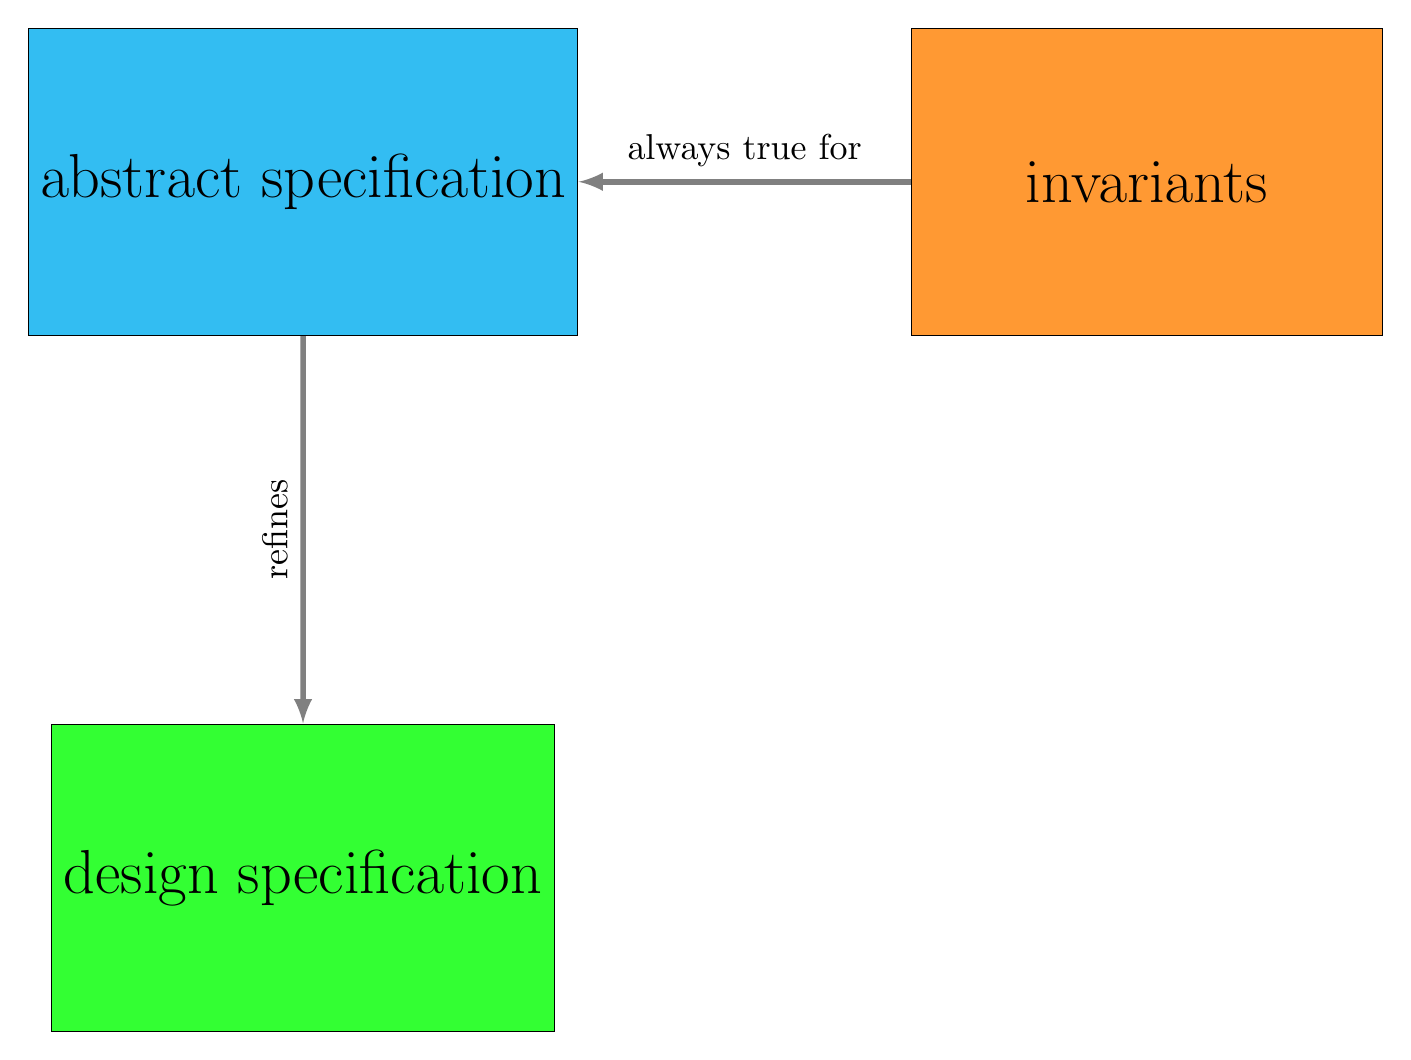
\begin{tikzpicture}[node distance=4cm, every node/.style={scale=1.3}]
        % styles
        \tikzstyle{cell} = [rectangle, minimum width=4.6cm, minimum height=3cm, text centered, draw=black]
        \tikzstyle{arrow} = [line width=2pt,->,>=latex,draw=gray]
        \tikzstyle{box} = [draw, rectangle, align=center, minimum width=11cm, inner sep=3ex]

        % wrap
        \node (abstract) [cell, fill=cyan!80] {\LARGE abstract specification};
        \node (invs) [cell, fill=orange!80, right=120pt of abstract] {\LARGE invariants};
        \node (design) [cell, fill=green!80, below=140pt of abstract] {\LARGE design specification};
        
        % \node [color=red] at (0, -150pt) {blocked access};
        % \node [color=green!200] at (-115pt, -180pt) {good access};

        % flow of information
        \draw [arrow] (abstract) -- (design) node[midway, left] {\rotatebox{90}{refines}};
        \draw [arrow] (invs) -- (abstract) node[midway, above] {always true for};
    \end{tikzpicture}
    \caption{Depiction of the proof architecture explored in this paper.
    A high-level description of what \lstinline{udp_wrap} should do
    is described in code in the abstract specification.
    An more concrete implementation which makes some assumptions about hardware
    is then defined in the design specification.
    Desirable qualities of \lstinline{udp_wrap} are described as invariants,
    which apply to the abstract specification.
    Lastly, a notion of program correspondence is shown between the
    abstract and design specification---namely, the design specification
    should refine the abstract specification.
    }
    \label{fig:network-stack}
\end{figure}

\section{Abstract specification}
\begin{lstlisting}[language=isabelle]
type_synonym message $=$ "nat list"

type_synonym ip_addr $=$ "nat"
type_synonym port $=$ "nat"
type_synonym socket $=$ "ip_addr $\times$ port"
type_synonym connection $=$ "socket $\times$ socket"

\end{lstlisting}
TODO: discuss.
Finally, a connection is uniquely identified by two sockets:
a source socket and a destination socket.
\begin{lstlisting}[language=isabelle]
definition udp_wrap :: "message $\Rightarrow$ connection $\Rightarrow$ message" where
  "udp_wrap msg conn $\equiv$ (let
                          src_sk $=$ src conn;
                          dst_sk $=$ dst conn;
                          src_ip_addr $=$ ip_addr src_sk;
                          dst_ip_addr $=$ ip_addr dst_sk;
                          src_port $=$ port src_sk;
                          dst_port $=$ port dst_sk;
                          len $=$ length msg $+$ udp_hdr_sz
                        in
                          [src_port, dst_port, len,
                           checksum16 [src_ip_addr,
                                       dst_ip_addr,
                                       0, udp_proto, len]
                          ]) $@$ msg"
\end{lstlisting}
TODO: discuss.
\begin{itemize}
    \item encoding in this case is prepending a header
    \item mention that the checksum can be omitted?
\end{itemize}



\section{Invariants}
% TODO: invariant singular?
\begin{lstlisting}[language=isabelle]
lemma compose_to_id:
"VARS orig_msg wrapped_msg unwrapped_msg conn
&\colorbox{green}{\{well\_formed orig\_msg conn\}}&
&\colorbox{cyan}{wrapped\_msg := udp\_wrap orig\_msg conn;}&
&\colorbox{cyan}{unwrapped\_msg := udp\_unwrap wrapped\_msg}&
&\colorbox{blue}{\{orig\_msg = unwrapped\_msg\}}&"
\end{lstlisting}

    This is a type of \textit{Hoare triple}, which are statements of the form
\begin{lstlisting}[language=isabelle]
&\colorbox{green}{\{precondition\}}&
&\colorbox{cyan}{program that changes state}&
&\colorbox{blue}{\{postcondition\}}&
\end{lstlisting}

\begin{itemize}
    \item mention that we can't prove this invariant yet, since we need
        to define unwrap?
    \item give some nice formal definitions of Hoare triples
        from semantics.
    \item discuss how the triples themselves can be composed to get bigger triples
    \item mention that this is from the HOL-Hoare library or whatever
\end{itemize}


\section{Design specification}
%TODO: remove the dot dot dots?
\begin{lstlisting}[language=isabelle]
type_synonym message_d = "byte list"

(* IPv6 addresses are 8 16-bit words *)
type_synonym ip_addr_d $=$ "word16 $\times$ word16 $\times \cdots \times$ word16"
type_synonym port_d $=$ "word16"
type_synonym socket_d $=$ "ip_addr_d $\times$ port_d"
type_synonym connection_d $=$ "socket_d $\times$ socket_d"
\end{lstlisting}
\begin{itemize}
    \item discuss word library
    \item show some of the helper definitions we made
    \item show some simps you can do to convert between
\end{itemize}

\begin{lstlisting}[language=isabelle]
definition udp_wrap_d :: "message_d $\Rightarrow$ connection_d $\Rightarrow$ message_d"
where "udp_wrap_d msg conn $\equiv$ (let
                            src_sk $=$ src conn;
                            dst_sk $=$ dst conn;
                            src_ip_addr $=$ ip_addr src_sk;
                            dst_ip_addr $=$ ip_addr dst_sk;
                            src_port $=$ port src_sk;
                            dst_port $=$ port dst_sk;
                            len $=$ (of_nat
                        (length msg $+$ udp_hdr_sz)::word16);
                            chksum $=$ (0 :: word16)
                          in
                            (porttomsgd src_port $@$
                             porttomsgd dst_port $@$
                             w16tomsg len $@$
                             w16tomsg chksum
                            ) $@$ msg)"


\end{lstlisting}
\begin{itemize}
    \item discuss isabelle definition vs fun vs inductive?
    \item minimally different on the surface from the abstract spec
    \item need to do appends ($@$ ) instead of cons ($\#$ ) due to 
        things getting split up (16-bit port to 2 8-bit numbers, for example)
\end{itemize}


\section{Refinement}

\section{Ongoing and future work}
\subsection{Convert C to Simpl}
\begin{itemize}
    \item show some example conversions
    \item discuss need to switch to more seL4 way of doing things?
\end{itemize}

\chapter{Conclusions}
\section{Conclusions}
\section{Future Work}
\begin{itemize}
    \item Make abstract and design specs for other layers
    \item c conversion for other layers
    \item c conversion for UDP?
    \item refinement for other layers
    \item seL4 proofs (specifically, PD stuff)
    \item introduce hardware problems
        \begin{itemize}
            \item think of this as relaxing assumptions about hardware
            \item e.g. packets won't be corrupted, but could arrive in weird orders
            \item note that there's probably a limit to this,
                since a packet could randomly corrupt to
                look completely legit---it's just very
                unlikely with all the error correction
                going on.
                Thus, we could model this by, e.g.,
                saying that only a limited arbitrary subset
                of the packet can be corrupted;
                or by saying any part of the packet other
                than the CRC can be corrupted.
                Pros/cons to each.
        \end{itemize}
    \item introduce linear temporal logic to have some ``always eventually''-type stuff
\end{itemize}
\section{Discussion}

\chapter{A Day in the Life of}
\begin{itemize}
    \item some isabelle guidelines
\end{itemize}


\section{Isabelle session management}
TODO: where to put this? Appendix?
At the root of your directory tree, a ``ROOTS'' file may be placed, which describes all directories with required sessions (see figure~\ref{fig:isabelle-roots-file}).
Each directory referred to in the ROOTS file must contain a ``ROOT'' file, which provides isabelle with the information for creating various sessions
(see figure~\ref{fig:isabelle-root-file-spec}).
Sessions in a particular ROOT file may refer to sessions in another, but with some restrictions.
In our example, the refinement session RefineAD deals with the abstract and design specifications, whose theories are contained in sessions
ASpec and DSpec.
Hence, our ROOTS file must contain a reference to both parent directories spec/ (which contains the files for both ASpec and DSpec), and proof/
(which contains the files for ADRefine).
Furthermore, the ADRefine session must explicitly list ASpec and DSpec as required parent sessions in its own ROOT file under proof/ (see figure~\ref{fig:isabelle-root-file-proof}).

\begin{figure}[htpb]
    \centering
    \begin{lstlisting}[language=file]
spec
proof
    \end{lstlisting}
    
    \caption{Example ROOTS file, assuming the root of the directory tree contains a single spec/ and proof/ folder.}
    \label{fig:isabelle-roots-file}
\end{figure}

\begin{figure}[htpb]
    \centering
    \begin{lstlisting}[language=isabelle]
session ASpec in "Aspec" = HOL +
  theories
    "Network_A"
    "Udp_A"

session DSpec in "Dspec" = HOL +
  sessions
    "HOL-Library"
  theories
    "Network_D"
    "Udp_D"
    \end{lstlisting}
    
    \caption{Example ROOT file in the spec/ directory. Two sessions are created: ASpec (an abstract specification) and DSpec (a design specification).}
    \label{fig:isabelle-root-file-spec}
\end{figure}

\begin{figure}[htpb]
    \centering
    \begin{lstlisting}[language=isabelle]
session RefineAD in "RefineAD" = HOL +
  sessions
    "ASpec"
    "DSpec"
  theories
    "Relation"
    \end{lstlisting}
    
    \caption{Example ROOT file in the proof/ directory. Note that the RefineAD session relies on the ASpec and DSpec sessions defined in a different ROOT file (in our case, located in the spec/ directory).}
    \label{fig:isabelle-root-file-proof}
\end{figure}


% If you want to include appendices, just use the \appendix command and then make chapters as normal
\appendix
\chapter{Installation notes}

See \url{https://www.overleaf.com/read/qyhckhfyfvmb} on Overleaf for useful examples of formatted text, typing in IPA, etc.

% For the bibliography style, I load `sp.bst', the style used by the LSA in the journal `Semantics and Pragmatics'. For how to include in-line citations with page numbers and other conventions, refer to nus-el-ht.sty. 
\backmatter
\bibliography{el-ht.bib}
\end{document}
